\documentclass[a4paper,12pt]{scrartcl}

\usepackage[a4paper,left=3.5cm,right=2.5cm,bottom=3.5cm,top=3cm]{geometry}

\usepackage{amsmath}
\usepackage{subfigure}
\usepackage{algorithm}
\usepackage{algorithmic}
%\numberwithin{algorithm}{document}
\usepackage[pdftex]{graphicx,color}

\usepackage{caption}
\usepackage{setspace}
\usepackage{fancyvrb}

\usepackage[pdftex,
		hyperindex=true,
		linktocpage=true,
		plainpages=false,
		pdfpagelabels]{hyperref}			% Clickbare Links im Dokument
\renewcommand{\figureautorefname}{Fig.}
\newcommand{\subfigureautorefname}{Fig.}
\hypersetup{colorlinks=true}
\hypersetup{citecolor=black}
\hypersetup{linkcolor=black}
\hypersetup{urlcolor=black}

\usepackage{hyperref}

\setlength\parindent{0pt}

%opening
\title{AtomViewer\\Short manual}
\author{Christoph Begau\footnote{E-Mail: christoph.begau@icams.rub.de}, ICAMS, Ruhr-Universitaet Bochum}
\date{2012}

\bibliographystyle{unsrt}

\begin{document}

\maketitle

\section{About AtomViewer}
AtomViewer is a visualization and analysis tool for atomistic simulations, primarily molecular dynamics simulations.
By characterization of the atomic configuration it can display or filter certain atoms, making crystal structures or other properties visible.
Plastic deformation in crystalline solids are mainly related to the creation and movement of dislocations. These entities are not directly part of atomistic simulations, but instead they need to be extracted from the atomistic configuration.
The detection and characterization of dislocations and their Burgers vector is one of the main features of AtomViewer, since it includes reference implementations for the dislocation network detection and classification methods as published by Begau et al.~\cite{Begau2011934,Begau2012}.

AtomViewer is open source software and is written in a way that it can be extended towards different materials and crystal structures as well as custom post-processing and rendering routines.
Build-in features support functionality for crystals in FCC, BCC and B2 structures. However, the algorithms to detect and characterize dislocations are not limited to these structures and can be extended to other materials and polycrystalline materials as well.

AtomViewer is not intended as an replacement for other MD visualization tools as AtomEye\footnote{\url{http://li.mit.edu/Archive/Graphics/A/}}, Ovito\footnote{\url{http://www.ovito.org/}}, VMD\footnote{\url{http://www.ks.uiuc.edu/Research/vmd/}} or many more, but as an addition to be used in certain applications.

\newpage
\section{System requirements}

AtomViewer requires 
\begin{itemize}
 \item{ an installed Java runtime enviroment version 6 or newer}
 \item{ a graphic device supporting OpenGL version 2.0 or higher}
 \item{ one of the supported operating systems: Microsoft Windows (XP-Win 7), Linux, MacOS, Solaris (each supported in 32- and 64-bit versions, not all platforms are tested) }
\end{itemize}

Please start AtomViewer by starting the included scripts
\begin{itemize}
 \item{AtomViewer.sh -- Linux, MacOS, Solaris}
 \item{AtomViewer.bat -- Windows}
\end{itemize}

Large atomistic data sets may require a large amount of memory. By default the maximum memory usage of AtomViewer is limited to about 1000~MB. If more memory is required, please modify the startup script. E.g.\ set the parameter``-Xmx4096M'' to increase the maximum memory to 4~GB. The possible maximum of memory that can be acquired depends on operating system, physical memory in the computer and the installed java virtual machine.

\begin{figure}[ht]
 \centering
 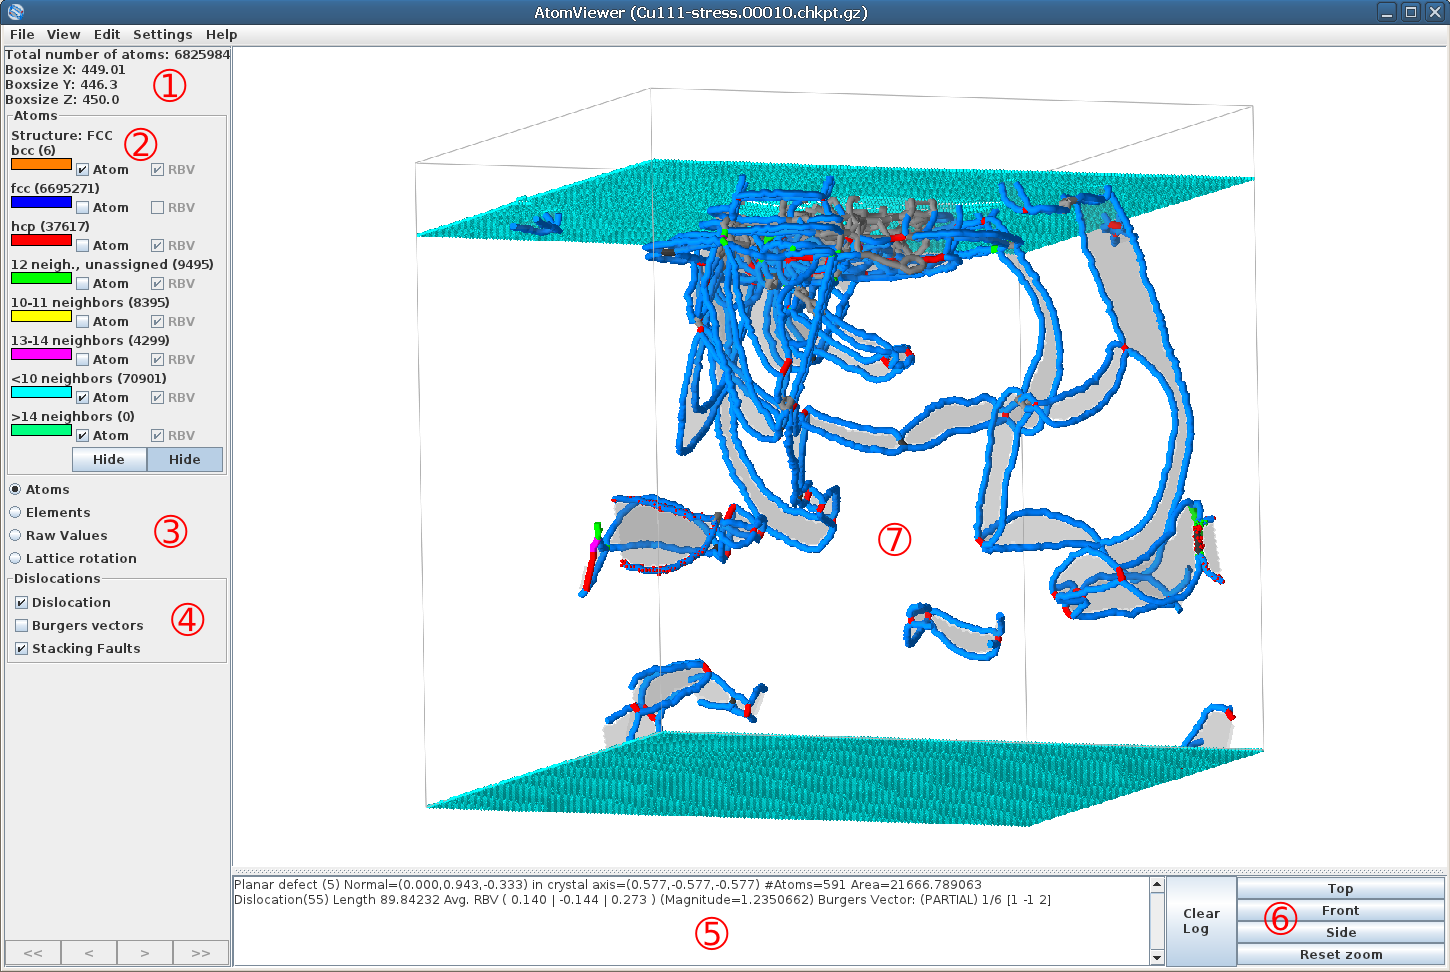
\includegraphics[width = 12cm]{./MainWindowNotes.png}
\captionsetup{singlelinecheck=off}
\caption[Titel]{Atom Viewer main window
\begin{scriptsize}
\begin{enumerate}
\item Information about the simulation volume and the number of imported atoms
\item Show/Hide the atoms assigned to certain classes and the resultant Burgers vector per atom (if available)
\item Different displaying styles for atomic information
\item Display the dislocation networks and (if available) stacking faults
\item Information for elements that are selected by clicking on them are printed to this log.
\item Select axis aligned perspectives. Holding down the Shift-key will clicking, results in selecting the opposite perspective.
\item Atoms and elements of microstructure are rendered here.
\end{enumerate}
\end{scriptsize}
}

\end{figure}

\section{Data format for import}
AtomViewer supports files in the IMD-format as decribed in

\url{http://www.itap.physik.uni-stuttgart.de/~imd/userguide/config.html}

For easier import, the files can even be more simple, a minimal file looks as followed:

\begin{Verbatim}[frame=single, samepage=true, numbers = left]
#F A
#C x y z
#X 3.520000 0 0
#Y 0 3.520000 0
#Z 0 0 3.520000
#E
2.636128 0.888096 0.891264
2.636128 2.648096 2.651264
0.876128 0.888096 2.651264
0.876128 2.648096 0.891264
\end{Verbatim}

Line~1 defines the file format (A=ASCII in this case), line~2 the type of each column (here x,y,z coordinate). Please note that only files with the order x y z are supported.
Line~3-5 define the simulation box size. Currently only orthogonal simulation boxes are supported. The origin of the simulation box is always at (0.0, 0.0, 0.0). Atoms outside the box are either placed inside the box in case of periodic boundary conditions or are imported and displayed but are ignored during most analysis operations in case of free boundaries.
The header must be closed with the sequence \#E.

Each following line defines the coordinate of an atom.
Besides the mandatory xyz-coordinates, additional predefined parameters are possible as given in the following table:

\begin{center}
\begin{tabular}{l|l|l}
Name & Format & Description\\
\hline
x y z & 3$\times$ float & atomic coordinate\\
number & integer & unique number of the atom\\
type & integer & identifier for the (virtual) element of the atom\\
\end{tabular}
\end{center}

An example file including all these features looks like this.
\begin{Verbatim}[frame=single, samepage=true, numbers = left]
#F A
#C number type x y z
#X 3.520000 0 0
#Y 0 3.520000 0
#Z 0 0 3.520000
#E
1 0 2.636128 0.888096 0.891264
2 0 2.636128 2.648096 2.651264
3 0 0.876128 0.888096 2.651264
4 0 0.876128 2.648096 0.891264
\end{Verbatim}

Additional custom columns can be imported using the editor under ``Edit->Edit configuration'' and providing the custom column keywords, a name and an optional unit.
The checkbox ``Raw values'' must be ticked when files to be opened are selected.
Files should either have the ending ``.chkpt'' or ``.ada'' to be imported directly. If a sequence of multiple files is to be opened they should be ending with ``.xxxxx.chkpt'' or ``.xxxxx.ada'' where xxxxx is a continuous sequence of numbers.
Files compressed with gzip can be opened directly. In this case the files need the additional suffix ``.gz'' at the end of the name.

Limited support for file from the Lammps MD code is implemented as well.

\begin{figure}[ht]
 \centering
 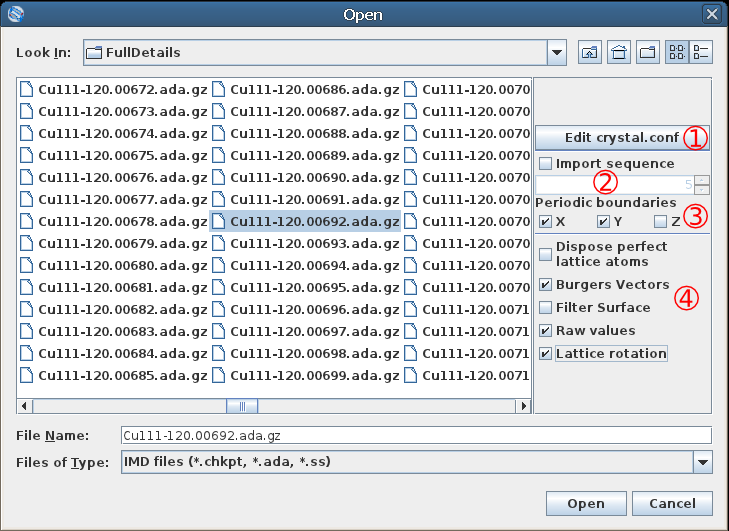
\includegraphics[width = 8cm]{./OpenDialogNotes.png}

\captionsetup{singlelinecheck=off}

\caption[Titel]{ Open dialog: Different options can be enable and disabled before opening files 
\begin{scriptsize}
\begin{enumerate}
\item Edit the crystal configuration (see Figure~\ref{fig:crystalConf}).
\item If the files are properly number it is possible to open a sequence of files by selecting the first file and the number of files. Otherwise multiple files can be selected. This feature is not available for LAMMPS files.
\item Enable periodic boundaries conditions in selected directions. For LAMMPS files, this setting is ignored if the boundary conditions are given in the file header.
\item Enable and disable different features of analysis
\end{enumerate}
\end{scriptsize}
}
\end{figure}

\paragraph{Crystal parameters}
Besides the atomic configuration, additional information concerning the crystal is needed to analyze the crystal properly.

The following information must be provided:
\begin{itemize}
 \item{the crystal structure (e.g.\ BCC or FCC)}
 \item{the lattice constant}
 \item{the crystal orientation}
\end{itemize}

Lattice constant and the crystal structure are required to identify defects correctly, where the crystal orientation is required to calculate Burgers vectors and lattice rotations correctly.
If the configuration file ``crystal.conf'' is not found in the same folder as the data, AtomViewer will ask for these information.

\textbf{Warning:} Do not place simulations of different materials or orientations in the same folder. Each of these simulations has to be in its own subfolder together with a proper configuration file.

\begin{figure}[ht]
 \centering
 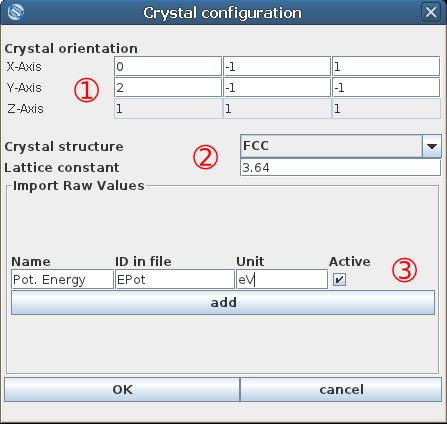
\includegraphics[width = 8cm]{./CrystalConfDialogNotes.png}

\captionsetup{singlelinecheck=off}

\caption[Titel]{Crystal.conf dialog: Define the crystal properties and imported fields here
\begin{scriptsize}
\begin{enumerate}
\item Define the crystal orientation in the Cartesian system. Axis x and y must be orthogonal, z is automatically computed.
\item Set crystal structure and lattice constant
\item Define additional values that are imported directly from the input file. ``Name'' defines the label that will be used for displaying the value. 
``ID in file'' must match the values ID used in the files to be imported. The unit is optional, if provided it will be added to values in the color bars.
Remove a value by unticking the ``Active'' checkbox. Add another value by clicking ``add''.
\end{enumerate}
\end{scriptsize}
}

 \label{fig:crystalConf}
\end{figure}

\section{Analysis features}

\paragraph{Defect state}

Defects are automatically detected with a modified bond angle analysis method (see \cite{BAD} and \cite{Begau2011934} for the modified version) if the column ``defectType'' is not found in the input files.
Depending on the configuration of the nearest neighbor atoms are assigned.

\begin{center}
\begin{table}
\caption*{FCC characterization}
\begin{tabular}{l|l|l}
ID & Description & Burgers vectors calculated\\
\hline
0 & BCC & no\\
1&FCC&yes\\
2&HCP&yes\\
3& 14 neighbors atoms, distorted order& yes\\
4& 12-13 neighbors & yes\\
5&15 neighbors&yes\\
6& Free surface, \textless11 neighbors & no\\
7& Unknown&yes\\
\end{tabular}
\end{table}
\end{center}

\begin{center}
\begin{table}
\caption*{BCC characterization}
\begin{tabular}{l|l|l}
ID & Description & Burgers vectors calculated\\
\hline
0 & BCC & yes\\
1&FCC&no\\
2&HCP&no\\
3& 12 neighbor atoms, distorted order & yes\\
4& \textless12 neighbors & yes\\
5&\textgreater12 neighbors&yes\\
6& Free surface, \textless10 neighbors & no\\
7& Unknown&yes\\
\end{tabular}
\end{table}
\end{center}

\paragraph{Resultant burgers vectors \& dislocation network}
Dislocation networks including Burgers vectors are computed if the option ``Burgers vectors'' is enabled during import.
Burgers vectors are computed via a modified version of the Nye-tensor analysis by Hartley\&Mishin (\cite{NyeTensor,NyeTensor2}). The derived resultant burgers vectors are combined into dislocation networks (\cite{Begau2011934}). Resultant burgers vectors are computed for each atom identified as certain defect types. 
If the crystal orientation is given correctly, the results of the dislocation network analysis are in most cases fairly accurate, but are prone to wrong classifications in the vicinity of free surfaces or defects like cracks.


\paragraph{Lattice rotations}
Per atom lattice rotations can be calculated in full atomic simulations. The rotations can be displayed either in degrees of rotation around the x-axis, y-axis or z-axis or as an absolute deviation angle.
For very severely distorted atoms the calculation can fail. In this case a rotation of zero is assigned.

\section{Output Formats}
Dislocation networks can be saved to be processed in other applications.
The output file consists of two sections. The first defines the number of nodes and their position. The second sections defines a dislocation per line as a sequence of nodes and the Burgers vector.
The three components of the Burgers vector are in crystal coordinates. If the Burgers vector has been identified, the line terminates with ``y''. If no Burgers vector has been identified the line terminates with ``n''. In this case either no Burgers vector has been identified at all or the numerical averaged resultant Burgers vector could not be mapped to a crystallographic possible one. The numerical value is then printed instead of the true burgers vector.

\begin{Verbatim}[frame=single, samepage=true, numbers = left]
#total number of nodes
209
#number x y z
0 155.61615 185.73717 219.36273
1 124.12319 162.65952 380.88416
2 126.55689 162.48555 380.7972
3 128.97746 162.46237 380.71375
4 135.29456 201.71378 382.6585
5 135.15097 207.23106 384.94006
....
#total number of dislocations
406
#number numberOfNodes n_1 n_2 ... n_n BV_x BV_y BV_z BV_identified
#BV_identified: (y) if Burgers vector is identified,
#(n) if just a numerical average is known
0 6 17528 17601 17695 17685 15752 17539 0.1667 -0.6667 0.1667 y
1 2 17840 17842 0.0000 0.0000 0.0000 n
3 2 17824 17833 0.0000 0.0000 0.0000 n
...
\end{Verbatim}


\section{Known limitations}
\paragraph{Dislocations in pseudo 3D simulation and infinitely long dislocations}
Dislocations are not properly identified in case the simulation box is very small and dislocations are infinite due to periodic boundaries. However, resultant Burgers vectors are correctly identified.
\paragraph{Rendering performance}
Default settings are fairly stable but slow. Improvements can be made by enabling ``instanced rendering'' in the settings menu. However, some AMD graphic cards produce a rather strange behavior with this option.

\paragraph{Enabling more features in AtomViewer}
AtomViewer contains several features that are either not well tested, are not usable in all crystal structures or rely on special data structures as for example grain- and phaseboundary approximations in its current state. These features are included in AtomViewer, but are not available by default. Additional functionality becomes available by unchecking ``Basic features only'' in the settings menu. Beware, additional features are likely not working in the way it is expected.

\section{License}
AtomViewer is free software: you can redistribute it and/or modify it under the terms of the GNU General Public License as published by the Free Software Foundation, either version 3 of the License, or (at your option) any later version.

AtomViewer is distributed in the hope that it will be useful, but WITHOUT ANY WARRANTY; without even the implied warranty of MERCHANTABILITY or FITNESS FOR A PARTICULAR PURPOSE.See the GNU General Public License for more details.

You should have received a copy of the GNU General Public License along  with AtomViewer. If not, see http://www.gnu.org/licenses/
AtomViewer's source code can be found embedded into the jar-file ``AtomViewer.jar''.


\bibliography{literature}
\end{document}